% This is samplepaper.tex, a sample chapter demonstrating the
% LLNCS macro package for Springer Computer Science proceedings;
% Version 2.20 of 2017/10/04
%
\documentclass[runningheads]{llncs}
%
\usepackage{array}
\usepackage{multirow}
\usepackage{wrapfig}
\usepackage{float}
\usepackage{svg}
\usepackage{colortbl}
\usepackage{pdflscape}
\usepackage{tabu}
\usepackage{threeparttable}
\usepackage{threeparttablex}
\usepackage[normalem]{ulem}
\usepackage{makecell}
\usepackage{xcolor}
\usepackage{longtable}
\usepackage{booktabs}
\usepackage{amssymb}
\usepackage{amsmath}
\usepackage{graphicx}
\usepackage[utf8]{inputenc}
\usepackage[hyphens]{url} % not crucial - just used below for the URL
\usepackage{hyperref}
\hypersetup{
    colorlinks=true,
    linkcolor=blue,
    filecolor=blue,
    urlcolor=blue,
}
\providecommand{\tightlist}{%
  \setlength{\itemsep}{0pt}\setlength{\parskip}{0pt}}
% Used for displaying a sample figure. If possible, figure files should
% be included in EPS format.


% Pandoc citation processing
\newlength{\cslhangindent}
\setlength{\cslhangindent}{1.5em}
\newlength{\csllabelwidth}
\setlength{\csllabelwidth}{3em}
\newenvironment{CSLReferences}[2] % #1 hanging-ident, #2 entry spacing
 {% don't indent paragraphs
  \setlength{\parindent}{0pt}
  % turn on hanging indent if param 1 is 1
  \ifodd #1 \everypar{\setlength{\hangindent}{\cslhangindent}}\ignorespaces\fi
  % set entry spacing
  \ifnum #2 > 0
  \setlength{\parskip}{#2\baselineskip}
  \fi
 }%
 {}
\usepackage{calc}
\newcommand{\CSLBlock}[1]{#1\hfill\break}
\newcommand{\CSLLeftMargin}[1]{\parbox[t]{\csllabelwidth}{#1}}
\newcommand{\CSLRightInline}[1]{\parbox[t]{\linewidth - \csllabelwidth}{#1}\break}
\newcommand{\CSLIndent}[1]{\hspace{\cslhangindent}#1}

\begin{document}
%
\title{Framework for ECG analysis\thanks{This work has been done under
the scope of - and funded by - the Ph.D.~Program in Health Data Science
of the Faculty of Medicine of the University of Porto, Portugal -
heads.med.up.pt}}
%
%\titlerunning{Abbreviated paper title}
% If the paper title is too long for the running head, you can set
% an abbreviated paper title here
%
%
\author{  Francisco Bischoff\inst{1,
2}\orcidID{0000-0002-5301-8672}\\  Pedro Pereira Rodrigues\inst{1,
2}\orcidID{0000-0001-7867-6682} }

\authorrunning{ Bischoff F., Rodrigues PP. }
% First names are abbreviated in the running head.
% If there are more than two authors, 'et al.' is used.
%
\institute{  \textsuperscript{1} Department of Community Medicine,
Information and Health Decision Sciences (MEDCIDS), Faculty of Medicine,
University of Porto, Porto, Portugal\\  \textsuperscript{2} Center for
Health Technology and Services Research (CINTESIS), Faculty of Medicine,
University of Porto, Porto, Portugal }

% \institute{truetrue}

\maketitle              % typeset the header of the contribution
%

\begin{abstract}
  Currently, Point-of-Care (POC) ECG monitoring works either as plot
  devices or alarms for abnormal cardiac rhythms using predefined normal
  trigger ranges and some rhythm analysis, which raises the problem of
  false alarms. In comparison, complex 12-derivation ECG machines are
  not suitable to use as simple monitors, and are used with strict
  techniques for formal diagnostics. We aim to identify, on streaming
  data, life-threatening hearth electric patterns to reduce the number
  of false alarms, using low CPU and memory maintaining robustness. The
  study design is comparable to a diagnostic study, where high accuracy
  is essential. Physionet's 2015 challenge yielded very good algorithms
  for reducing false alarms. However, none of the authors reported
  benchmarks, memory usage, robustness test, or context invariance that
  could assure its implementation on real monitors to reduce alarm
  fatigue indeed. We expect to identify the obstacles of detecting
  life-threatening ECG changes within memory, space, and CPU constraints
  and to reduce ECG monitor's false alarms using the proposed
  methodology, and assess the feasibility of implementing the algorithm
  in the real world and other settings than ICU monitors.

  \keywords{
        anomaly detection \and
        ECG \and
        fading factors \and
        matrix profile \and
        time series \and
        point-of-care  }

\end{abstract}
%
%
% \def\spacingset#1{\renewcommand{\baselinestretch}%
% {#1}\small\normalsize} \spacingset{1}

\hypertarget{introduction}{%
\section{Introduction}\label{introduction}}

Point-of-Care (POC) ECG monitoring works either as plot devices or
alarms for abnormal cardiac rhythms using predefined normal trigger
ranges. Modern devices also incorporate algorithms to analyze
arrhythmias improving their specificity. On the other hand, full
12-derivation ECG machines are complex, are not suited to use as simple
monitors, and are used with strict techniques for formal diagnostics of
hearth electric conduction pathologies. The automatic diagnostics are
derived from a complete analysis of the 12-dimension data after fully
and well collected. Both systems do not handle disconnected leads and
patient's motions, being strictly necessary to have a good and stable
signal to allow proper diagnosis. These interferences with the data
collection frequently originate false alarms increasing both patient and
staff's stress; depending on how it is measured, the rate of false
alarms (overall) in ICU is estimated at 65 to
95\%{[}\protect\hyperlink{ref-donchin2002}{11}{]}.

Alarm fatigue is a well-known problem that consists of a sensory
overload of nurses and clinicians, resulting in desensitization to
alarms and missed alarms (the ``crying wolf'' situation). Patient deaths
have been attributed to alarm
fatigue{[}\protect\hyperlink{ref-sendelbach2013}{23}{]}. In 1982 it was
recognized the increase in alarms with ``no end in sight''; studies have
demonstrated that most alarm signals have no clinical relevance and lead
to clinical personnel's delayed response. Ultimately patient deaths were
reported related to inappropriate responses to
alarms{[}\protect\hyperlink{ref-sendelbach2013}{23}{]}.

In April of 2013, The Joint
Commission{[}\protect\hyperlink{ref-the_jc}{4}{]} issued the Sentinel
Event Alert{[}\protect\hyperlink{ref-JointCommission2013}{16}{]},
establishing alarm system safety as a top hospital priority in the
National Patient Safety Goal. Nowadays (2021), this subject is still on
their list, in fourth place of
importance{[}\protect\hyperlink{ref-the_jc2021}{5}{]}.

In February 2015, the CinC/Physionet Challenge 2015 was about ``Reducing
False Arrhythmia Alarms in the
ICU{[}\protect\hyperlink{ref-Lawless1994}{19}{]}.

Due to this matter's importance, this research aims to identify abnormal
hearth electric patterns using streaming data, specifically those who
are life-threatening, reducing the false alarms, being a reliable signal
for Intensive Care Units to respond quickly to those situations.

\hypertarget{objectives-and-the-research-question}{%
\section{Objectives and the research
question}\label{objectives-and-the-research-question}}

This research aims to identify, on streaming data, abnormal hearth
electric patterns, specifically those which are life-threatening, to be
a reliable signal for Intensive Care Units to respond quickly to those
situations. It also may be able to continuously analyze new data and
correct itself shutting off false alarms.

As it is known, this goal is not a new problem, so the main questions to
solve are: (1) Can we reduce the number of false alarms in the ICU
setting? (2) Can we accomplish this objective using a minimalist
approach (low CPU, low memory) while maintaining robustness? (3) Can
this approach be used in other health domains other than ICU or ECG?

\hypertarget{related-works}{%
\section{Related Works}\label{related-works}}

The CinC/Physionet Challenge 2015 produced several papers aiming to
reduce false alarms on their dataset. In Table \ref{tab:alarms} it is
listed the five life-threatening alarms present in their dataset.

\begin{table}

\caption{\label{tab:alarms}Definition of the 5 alarm types used in CinC/Physionet Challenge 2015 challenge.}
\centering
\begin{tabu} to \linewidth {>{\raggedright\arraybackslash}p{5cm}>{\raggedright}X}
\toprule
\textbf{Alarm} & \textbf{Definition}\\
\midrule
Asystole & No QRS for at least 4 seconds\\
Extreme Bradycardia & Heart rate lower than 40 bpm for 5 consecutive beats\\
Extreme Tachycardia & Heart rate higher than 140 bpm for 17 consecutive beats\\
Ventricular Tachycardia & 5 or more ventricular beats with heart rate higher than 100 bpm\\
Ventricular Flutter/Fibrillation & Fibrillatory, flutter, or oscillatory waveform for at least 4 seconds\\
\bottomrule
\end{tabu}
\end{table}

They used as score the following formula, which penalizes five times the
false negatives (since we do not want to miss any real event):

\[Score=\frac{TP+TN}{TP+TN+FP+5*FN}\]

The five-best scores in this challenge are presented on Table
\ref{tab:scores}{[}\protect\hyperlink{ref-couto2015}{10},
\protect\hyperlink{ref-fallet2015}{12},
\protect\hyperlink{ref-hoogantink2015}{15},
\protect\hyperlink{ref-kalidas2015}{17},
\protect\hyperlink{ref-plesinger2015}{21}{]}.

\begin{table}

\caption{\label{tab:scores}Challenge Results on Streaming}
\centering
\begin{tabu} to \linewidth {>{\centering}X>{\raggedright\arraybackslash}p{9cm}}
\toprule
\textbf{Score} & \textbf{Authors}\\
\midrule
81.39 & Filip Plesinger, Petr Klimes, Josef Halamek, Pavel Jurak\\
79.44 & Vignesh Kalidas\\
79.02 & Paula Couto, Ruben Ramalho, Rui Rodrigues\\
76.11 & Sibylle Fallet, Sasan Yazdani, Jean-Marc Vesin\\
75.55 & Christoph Hoog Antink, Steffen Leonhardt\\
\bottomrule
\end{tabu}
\end{table}

Their algorithm did a pretty good job on the Physionet test set.
However, independently of their approach to this problem, none of the
authors reported benchmarks, memory usage, robustness test, or context
invariance that could assure its implementation on real monitors to
reduce alarm fatigue indeed.

There are other arrhythmias that this challenge did not assess, like
atrial standstill (hyperkalemia), third-degree atrioventricular block,
and others that may be life-threatening in some settings. Pulseless
electrical activity is a frequent condition in cardiac arrest but cannot
be identified without blood pressure information. This information is
usually present in ICU settings but not in other locations.

\hypertarget{the-planned-approach-and-methods-for-solving-the-problem}{%
\section{The planned approach and methods for solving the
problem}\label{the-planned-approach-and-methods-for-solving-the-problem}}

\hypertarget{state-of-the-art}{%
\subsection{State of the art}\label{state-of-the-art}}

A literature review of the last ten years is being conducted to assess
state of the art for ECG automatic processing collecting the following
points if available : (1) The memory and space used to perform the
primary goal of the algorithm (sound an alarm, for ex.). (2) The type of
algorithms used to identify ECG anomalies. (3) The type of algorithms
used to identify specific diagnoses (like a flutter, hyperkalemia, and
others). (4) Their performance (accuracy, ROC, etc.)

A broad search will be conducted on Pubmed, Scopus, Google Scholar,
device manuals, and other specific sources.

Keywords:

\begin{itemize}
\tightlist
\item
  ECG AND monitoring AND ICU
\item
  ECG AND {[} time series {]}
\item
  ECG AND automatic AND interpretation
\end{itemize}

Articles published after ``The PhysioNet/Computing in Cardiology
Challenge 2015: Reducing False Arrhythmia Alarms in the ICU'' will also
be analyzed.

\hypertarget{research-plan-and-methods}{%
\subsection{Research plan and methods}\label{research-plan-and-methods}}

This research is being conducted using the Research Compendium
principles{[}\protect\hyperlink{ref-compendium2019}{3}{]}:

\begin{enumerate}
\def\labelenumi{\arabic{enumi}.}
\tightlist
\item
  Stick with the convention of your peers;
\item
  Keep data, methods, and output separated;
\item
  Specify your computational environment as clearly as you can.
\end{enumerate}

Data management follows the FAIR principle (findable, accessible,
interoperable, reusable){[}\protect\hyperlink{ref-wilkinson2016}{24}{]}.

Currently, the dataset used is stored on a public
repository{[}\protect\hyperlink{ref-franz_dataset}{6}{]}, the source
code is publicly open and stored on
Github{[}\protect\hyperlink{ref-franz_github}{1}{]}, while the reports
and reproducibility information on each step is found on a public
website{[}\protect\hyperlink{ref-franz_website}{2}{]}. The current
dataset and further collected data will be publicly available following
the FAIR principle.

\hypertarget{type-of-study}{%
\subsubsection{Type of study}\label{type-of-study}}

This thesis will be a diagnostic study as the algorithm must classify
the change in pattern as positive or negative for life-threatening.

\hypertarget{the-data}{%
\subsubsection{The data}\label{the-data}}

Initially, we will use the CinC/Physionet Challenge 2015 dataset that is
publicly available on Physionet. This dataset is a good start for
exploring the primary goal of reducing false alarms. This dataset has
been curated for this challenge, and the events were labeled by experts,
so it is not raw data. All signals have been resampled (using anti-alias
filters) to 12 bits, 250 Hz, and have had FIR band-pass {[}0.05 to
40Hz{]} and mains notch filters applied to remove noise. Pacemaker and
other artifacts may be present on the
ECG{[}\protect\hyperlink{ref-Clifford2015}{9}{]}. Furthermore, this
dataset contains at least two ECG derivations and one or more variables
like arterial blood pressure, photoplethysmograph readings, and
respiration movements.

These variables may or may not be helpful for increasing the sensitivity
or specificity of the algorithm. We plan to use the minimum set of
variables as it is known in multi-dimensional analysis that using just
two (or some small subset) of all the dimensions can be much more
accurate than using all dimensions or a single
dimension{[}\protect\hyperlink{ref-gharghabi2018}{14}{]}.

At first, we will assemble a workflow to explore the Physionet's dataset
and find a suitable solution for detecting regime changes and verify if
these changes are, in fact, clinical changes or just artifacts. At this
stage, the aim is to build a classifier for the ``simplest'' type of
change: Asystole. While one may think detecting the ``absence'' of
heartbeats may be trivial, this will set the grounds for distinguishing
patient data from artifacts.

It is desirable that real data extracted from Portuguese ICU could be
used in a further stage to assess the validity of the model in real
settings and robustness (using raw data instead of filtered data). The
variables available on Physionet's dataset are commonly available on
Portuguese ICUs. However, this real data also need to go through several
stages, including manual labeling, which can hold back this project. In
addition to the dataset used on Challenge 2015, Physionet has a vast
collection of ECG recordings well labeled and reviewed by cardiologists.
Therefore, these data can be used as a final test for the resulting
model.

\hypertarget{workflow-management}{%
\subsubsection{Workflow management}\label{workflow-management}}

All steps of the process will be managed using the R package
\texttt{targets}{[}\protect\hyperlink{ref-landau2021}{18}{]} from data
extraction to the final report, as shown in Fig. \ref{fig:targets}.

\begin{figure}
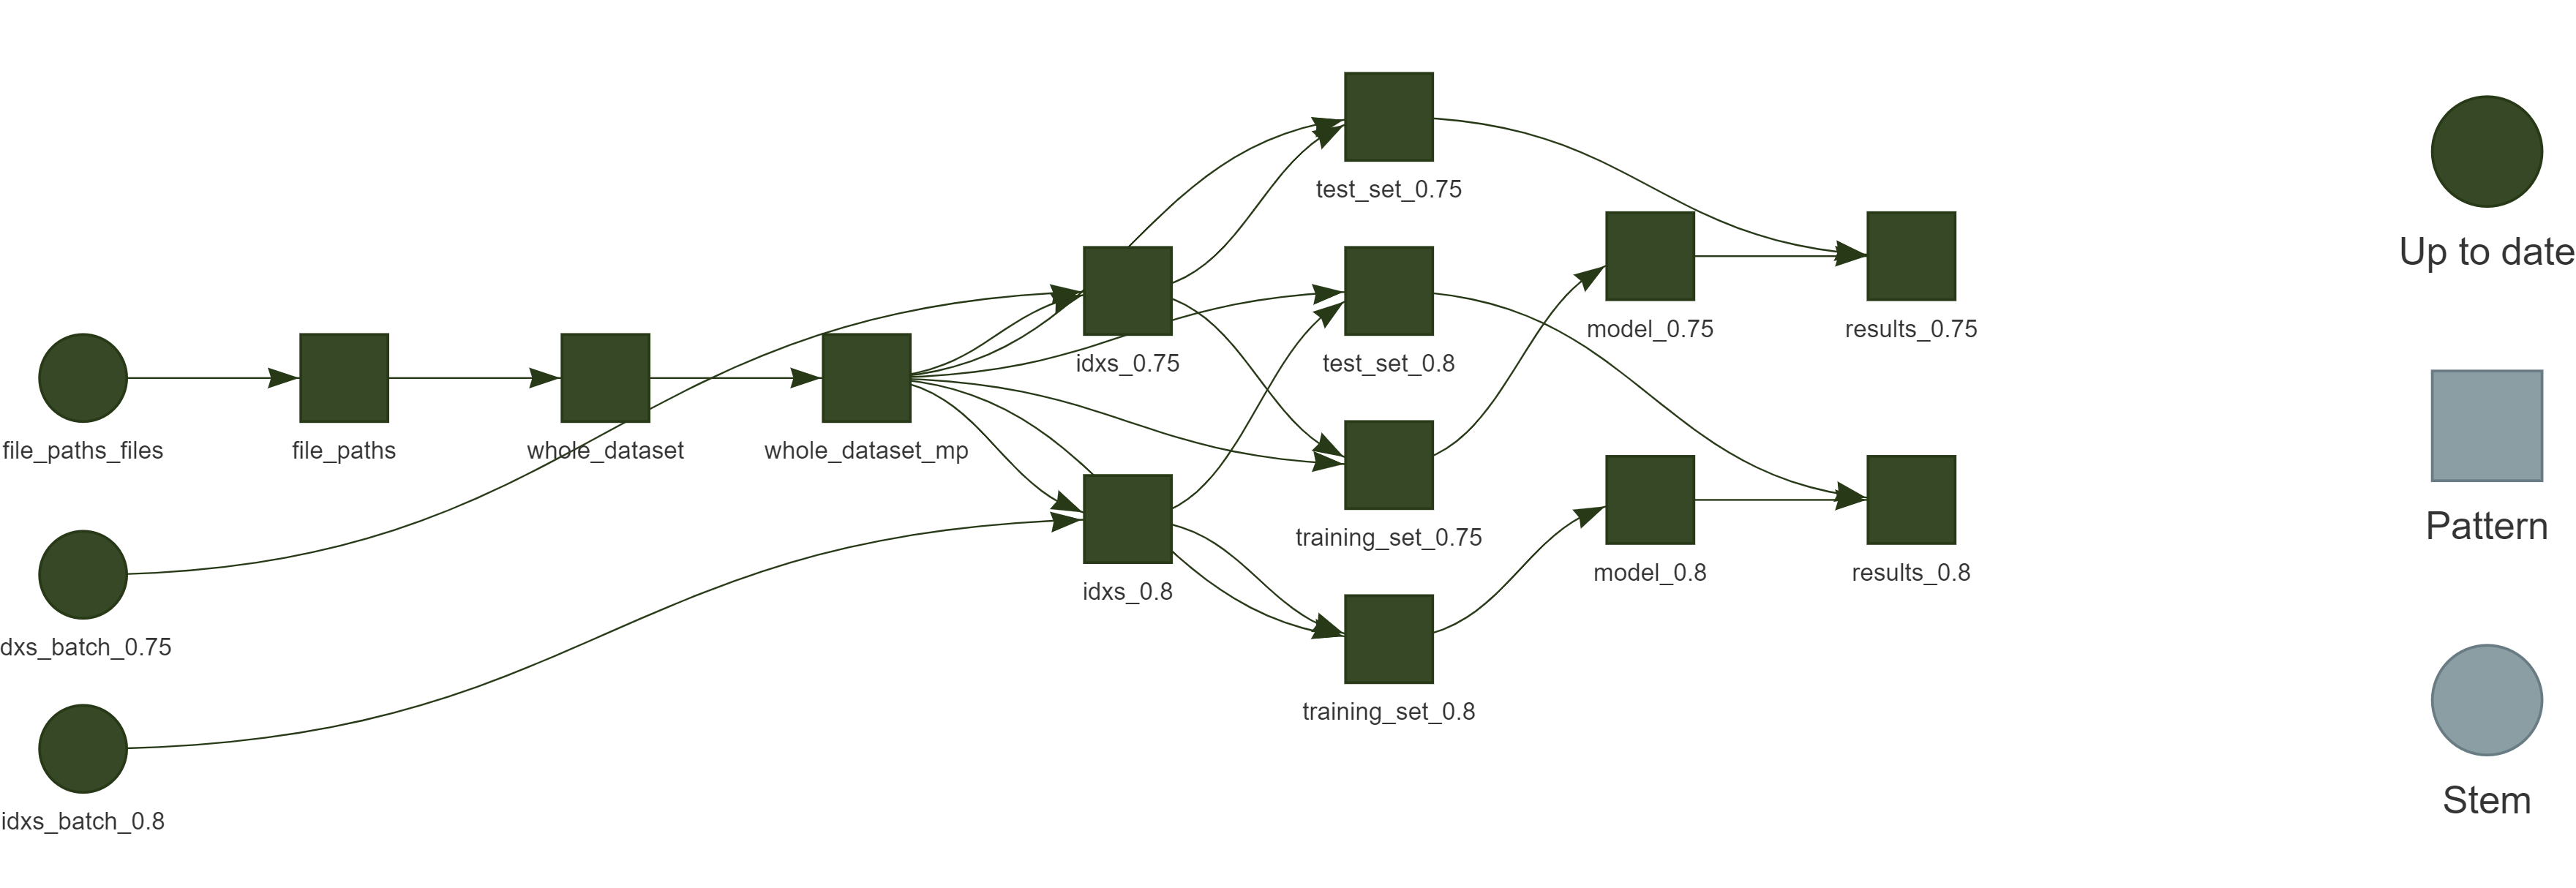
\includegraphics[width=1\linewidth]{targets} \caption{Reproducible research workflow using `targets`.}\label{fig:targets}
\end{figure}

The report will then be available on the main
webpage{[}\protect\hyperlink{ref-franz_website}{2}{]}, allowing
inspection of previous versions managed by the R package
\texttt{workflowr}{[}\protect\hyperlink{ref-workflowr2021}{7}{]}, as we
can see in Fig. \ref{fig:workflow_workflowr}.

\begin{figure}

\includegraphics[width=1\linewidth]{workflowr} \caption{Reproducible reports using `workflowr.`}\label{fig:workflow_workflowr}
\end{figure}

\hypertarget{proposed-approach}{%
\subsubsection{Proposed approach}\label{proposed-approach}}

The proposed approach is depicted in Fig. \ref{fig:workflow_image}. That
is only a draft of the final workflow. The algorithm for the
classification of the regime changes is still to be defined. However,
the main innovation resides in the correct regime detection. Also, to
achieve the goal of low CPU and memory usage, the strategy will be to
combine fading factors{[}\protect\hyperlink{ref-Gama2013}{13},
\protect\hyperlink{ref-Rodrigues2010}{22}{]} to reduce computation in
online settings like in this research.

\begin{figure}
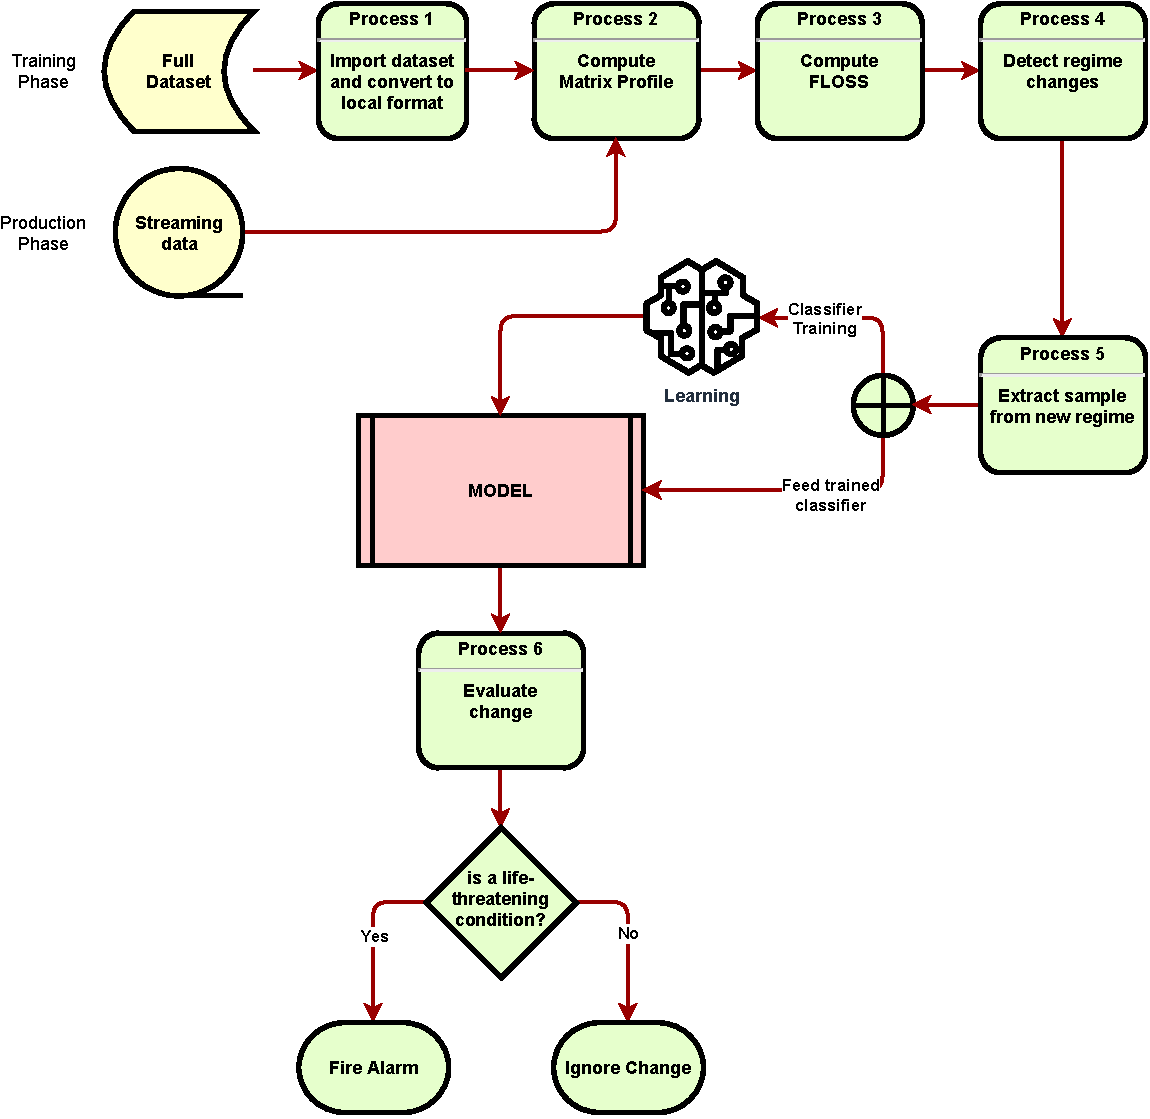
\includegraphics[width=1\linewidth]{false_alarm} \caption{Proposed approach to train the model for relevant patterns detection.}\label{fig:workflow_image}
\end{figure}

\hypertarget{statistical-analysis}{%
\subsubsection{Statistical analysis}\label{statistical-analysis}}

The Statistical analysis will be performed using R language v4.1.1 or
greater, and it will be computed the ROC curve for the algorithm.

The experiment will be conducted using the Matrix Profile
concept{[}\protect\hyperlink{ref-yeh2016}{25}{]}, the state-of-the-art
for time series analysis. It will be conducted several experiments to
identify the best algorithm for this task. One of such algorithms is the
online semantic segmentation for multi-dimensional time
series{[}\protect\hyperlink{ref-gharghabi2018}{14}{]}.

In addition, we will combine the fading
factors{[}\protect\hyperlink{ref-Gama2013}{13},
\protect\hyperlink{ref-Rodrigues2010}{22}{]} strategy to minimize the
memory and space consumption lowering the processor power needed,
allowing this algorithm to be used in almost any device.

\hypertarget{research-team}{%
\subsubsection{Research Team}\label{research-team}}

\begin{itemize}
\tightlist
\item
  Thesis Author: Francisco Bischoff
\item
  Supervisor: Professor Pedro Pereira Rodrigues
\item
  Co-supervisor: Professor Eamonn Keogh (UCR, Riverside)
\end{itemize}

\hypertarget{expected-results-and-outcomes}{%
\subsection{Expected results and
outcomes}\label{expected-results-and-outcomes}}

We expect the following results: (1) Identify the obstacles of
identifying life-threatening ECG changes within memory, space, and CPU
constraints. (2) Be able to reduce ECG monitor's false alarms using the
proposed methodology. (3) Assess the feasibility of implementing the
algorithm in the real world and other settings than ICU monitors.

And outcomes: (1) To achieve a better score of false alarm reduction
than the best on Physionet's 2015 challenge. (2) To push forward the
state-of-the-art technology on false alarms reduction, maybe even being
domain agnostic. (3) To draw more attention to fading factors as a
reliable, fast, and cheap approximation of the true value. (4) To draw
more attention to the matrix profile concept as an efficient, agnostic,
and almost parameter-free way to analyze time series. (5) To draw more
attention of the Patient Monitorization industry on solving the false
alarm problem.

\hypertarget{references}{%
\section*{References}\label{references}}
\addcontentsline{toc}{section}{References}

\hypertarget{refs}{}
\begin{CSLReferences}{0}{0}
\leavevmode\vadjust pre{\hypertarget{ref-franz_github}{}}%
\CSLLeftMargin{1. }
\CSLRightInline{Franzbischoff/false.alarm: PhD programme in health data
science, \url{https://github.com/franzbischoff/false.alarm}, last
accessed 2021/04/08.}

\leavevmode\vadjust pre{\hypertarget{ref-franz_website}{}}%
\CSLLeftMargin{2. }
\CSLRightInline{Franzbischoff/false.alarm: Reproducible reports,
\url{https://franzbischoff.github.io/false.alarm}, last accessed
2021/04/08.}

\leavevmode\vadjust pre{\hypertarget{ref-compendium2019}{}}%
\CSLLeftMargin{3. }
\CSLRightInline{Research compendium,
\url{https://research-compendium.science}, last accessed 2021/04/08.}

\leavevmode\vadjust pre{\hypertarget{ref-the_jc}{}}%
\CSLLeftMargin{4. }
\CSLRightInline{The joint commission,
\url{https://www.jointcommission.org}, last accessed 2021/04/08.}

\leavevmode\vadjust pre{\hypertarget{ref-the_jc2021}{}}%
\CSLLeftMargin{5. }
\CSLRightInline{The joint commission - national patient safety goals,
\url{https://www.jointcommission.org/standards/national-patient-safety-goals/hospital-national-patient-safety-goals/},
last accessed 2021/04/08.}

\leavevmode\vadjust pre{\hypertarget{ref-franz_dataset}{}}%
\CSLLeftMargin{6. }
\CSLRightInline{The PhysioNet computing in cardiology challenge 2015 -
dataset, \url{https://zenodo.org/record/4634013}, last accessed
2021/04/08.}

\leavevmode\vadjust pre{\hypertarget{ref-workflowr2021}{}}%
\CSLLeftMargin{7. }
\CSLRightInline{Blischak, J.D. et al.: Creating and sharing reproducible
research code the workflowr way {[}version 1; peer review: 3
approved{]}. F1000Research. 8, 1749, (2019).
\url{https://doi.org/10.12688/f1000research.20843.1}.}

\leavevmode\vadjust pre{\hypertarget{ref-Chambrin2001}{}}%
\CSLLeftMargin{8. }
\CSLRightInline{Chambrin, M.C.: Alarms in the intensive care unit: How
can the number of false alarms be reduced? Critical care (London,
England). 5, 4, 184--8 (2001). \url{https://doi.org/10.1186/cc1021}.}

\leavevmode\vadjust pre{\hypertarget{ref-Clifford2015}{}}%
\CSLLeftMargin{9. }
\CSLRightInline{Clifford, G.D. et al.: The PhysioNet/computing in
cardiology challenge 2015: Reducing false arrhythmia alarms in the ICU.
In: Computing in cardiology. (2015).
\url{https://doi.org/10.1109/cic.2015.7408639}.}

\leavevmode\vadjust pre{\hypertarget{ref-couto2015}{}}%
\CSLLeftMargin{10. }
\CSLRightInline{Couto, P. et al.: 2015 computing in cardiology
conference (CinC). Presented at the September (2015).
\url{https://doi.org/10.1109/cic.2015.7411019}.}

\leavevmode\vadjust pre{\hypertarget{ref-donchin2002}{}}%
\CSLLeftMargin{11. }
\CSLRightInline{Donchin, Y., Seagull, F.J.: The hostile environment of
the intensive care unit. Current Opinion in Critical Care. 8, 4,
316--320 (2002).
\url{https://doi.org/10.1097/00075198-200208000-00008}.}

\leavevmode\vadjust pre{\hypertarget{ref-fallet2015}{}}%
\CSLLeftMargin{12. }
\CSLRightInline{Fallet, S. et al.: 2015 computing in cardiology
conference (CinC). Presented at the September (2015).
\url{https://doi.org/10.1109/cic.2015.7408640}.}

\leavevmode\vadjust pre{\hypertarget{ref-Gama2013}{}}%
\CSLLeftMargin{13. }
\CSLRightInline{Gama, J. et al.: {On evaluating stream learning
algorithms}. Machine Learning. 90, 3, 317--346 (2013).
\url{https://doi.org/10.1007/s10994-012-5320-9}.}

\leavevmode\vadjust pre{\hypertarget{ref-gharghabi2018}{}}%
\CSLLeftMargin{14. }
\CSLRightInline{Gharghabi, S. et al.: Domain agnostic online semantic
segmentation for multi-dimensional time series. Data Mining and
Knowledge Discovery. 33, 1, 96--130 (2018).
\url{https://doi.org/10.1007/s10618-018-0589-3}.}

\leavevmode\vadjust pre{\hypertarget{ref-hoogantink2015}{}}%
\CSLLeftMargin{15. }
\CSLRightInline{Hoog Antink, C., Leonhardt, S.: 2015 computing in
cardiology conference (CinC). Presented at the September (2015).
\url{https://doi.org/10.1109/cic.2015.7408642}.}

\leavevmode\vadjust pre{\hypertarget{ref-JointCommission2013}{}}%
\CSLLeftMargin{16. }
\CSLRightInline{Joint Commission: {Sentinel event alert - Medical device
alarm safety in hospitals.} 50, 1--3 (2013).
\url{https://www.ncbi.nlm.nih.gov/pubmed/23767076}.}

\leavevmode\vadjust pre{\hypertarget{ref-kalidas2015}{}}%
\CSLLeftMargin{17. }
\CSLRightInline{Kalidas, V., Tamil, L.S.: 2015 computing in cardiology
conference (CinC). Presented at the September (2015).
\url{https://doi.org/10.1109/cic.2015.7411015}.}

\leavevmode\vadjust pre{\hypertarget{ref-landau2021}{}}%
\CSLLeftMargin{18. }
\CSLRightInline{Landau, W. et al.: Ropensci/targets, dynamic
function-oriented 'make'-like declarative workflows. Zenodo (2021).
\url{https://doi.org/10.5281/ZENODO.4062936}.}

\leavevmode\vadjust pre{\hypertarget{ref-Lawless1994}{}}%
\CSLLeftMargin{19. }
\CSLRightInline{Lawless, S.T.: Crying wolf: False alarms in a pediatric
intensive care unit. Critical care medicine. 22, 6, 981--5 (1994).
\url{https://www.ncbi.nlm.nih.gov/pubmed/8205831}.}

\leavevmode\vadjust pre{\hypertarget{ref-Parthasarathy2004}{}}%
\CSLLeftMargin{20. }
\CSLRightInline{Parthasarathy, S., Tobin, M.J.: Sleep in the intensive
care unit. Intensive Care Medicine. 30, 2, 197--206 (2004).
\url{https://doi.org/10.1007/s00134-003-2030-6}.}

\leavevmode\vadjust pre{\hypertarget{ref-plesinger2015}{}}%
\CSLLeftMargin{21. }
\CSLRightInline{Plesinger, F. et al.: 2015 computing in cardiology
conference (CinC). Presented at the September (2015).
\url{https://doi.org/10.1109/cic.2015.7408641}.}

\leavevmode\vadjust pre{\hypertarget{ref-Rodrigues2010}{}}%
\CSLLeftMargin{22. }
\CSLRightInline{Rodrigues, P.P. et al.: {Memoryless Fading Windows in
Ubiquitous Settings}. In: Proceedings of the first ubiquitous data
mining workshop. pp. 23--27 (2010).}

\leavevmode\vadjust pre{\hypertarget{ref-sendelbach2013}{}}%
\CSLLeftMargin{23. }
\CSLRightInline{Sendelbach, S., Funk, M.: Alarm Fatigue. AACN Advanced
Critical Care. 24, 4, 378--386 (2013).
\url{https://doi.org/10.4037/nci.0b013e3182a903f9}.}

\leavevmode\vadjust pre{\hypertarget{ref-wilkinson2016}{}}%
\CSLLeftMargin{24. }
\CSLRightInline{Wilkinson, M.D. et al.: The FAIR Guiding Principles for
scientific data management and stewardship. Scientific Data. 3, 1,
(2016). \url{https://doi.org/10.1038/sdata.2016.18}.}

\leavevmode\vadjust pre{\hypertarget{ref-yeh2016}{}}%
\CSLLeftMargin{25. }
\CSLRightInline{Yeh, C.-C.M. et al.: 2016 IEEE 16th international
conference on data mining (ICDM). Presented at the December (2016).
\url{https://doi.org/10.1109/icdm.2016.0179}.}

\end{CSLReferences}

\end{document}
